\chapter{Resumo Estendido em Língua Portuguesa}\label{appendix:pt_estendido}
\begin{singlespace}
{\setfonttimes\normalsize\noindent{\textbf{T\'{i}tulo:} \tituloportuguesnome}}\\
{\setfonttimes\normalsize{\textbf{Autor:} \autorinome}}\\
\ifthenelse{\equal{\autoriinome}{}}{}{\setfonttimes\normalsize{\textbf{Autor:} \autoriinome}\\}
\ifthenelse{\equal{\autoriiinome}{}}{}{\setfonttimes\normalsize{\textbf{Autor:} \autoriiinome}\\}
{\setfonttimes\normalsize{\textbf{Orientador:} \orientadornome}}\\
\ifthenelse{\equal{\corientadornome}{}}{}{\setfonttimes\normalsize{\textbf{Coorientador:} \corientadornome}\\}
{\setfonttimes\normalsize{\textbf{Programa de Pós-Graduação em \programadoaluno}}\\}
{\setfonttimes\normalsize{\textbf{Bras\'ilia, \dianome\ de \MakeLowercase{\mesnome}\ de \anonome}}\\\\}
{\setfonttimes\normalsize\noindent{\textbf{Palavras-chave:} \palavraschavecatalogoinome,~\palavraschavecatalogoiinome,~\palavraschavecatalogoiiinome,~\palavraschavecatalogoivnome.}}
\end{singlespace}
\vspace{-5mm}
\begin{otherlanguage}{portuguese}
\subsection*{Contextualização}
Figuras e tabelas podem ser utilizadas, mas lembre-se de usar "[]" após o "caption" and antes do "{}" para evitar que esta figura vá para a lista de figuras.

\begin{figure}[H]
	\centering %
	\scriptsize %
	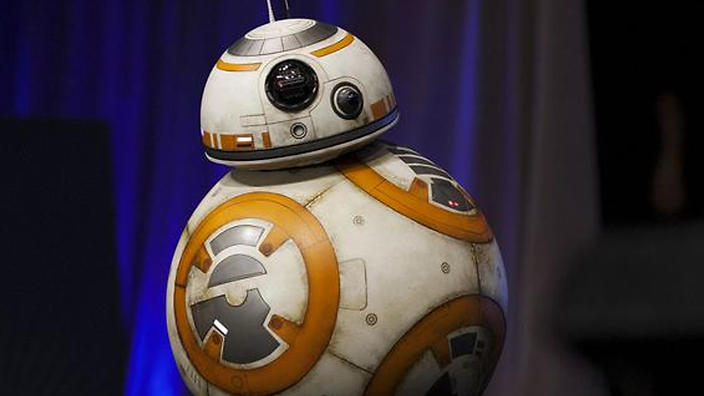
\includegraphics[width=\columnwidth]{new-bot}
	\caption[]{Este robô novamente!}
	\label{fig:appendix_oldbot}
\end{figure}
\subsection*{Metodologia}
Avaliou-se o blablabla
\subsection*{Resultados}
Os resultados foram muito bons...
\subsection*{Conclusão}
Escreva aqui as conclusões em português.
\end{otherlanguage}